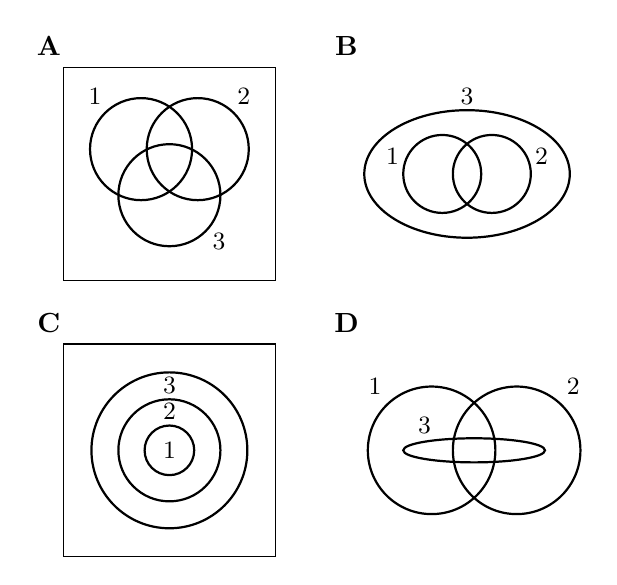
\begin{tikzpicture}[font=\small, scale=0.9]
% ---------- A: generic position inside a box X ----------
\begin{scope}
  \node[font=\bfseries] at (-0.2,3.3) {A};
  \draw (0,0) rectangle (3,3);
  \draw[thick] (1.1,1.85) circle (0.72);
  \draw[thick] (1.9,1.85) circle (0.72);
  \draw[thick] (1.5,1.2) circle (0.72);
  \node at (0.45,2.6) {1};
  \node at (2.55,2.6) {2};
  \node at (2.2,0.55) {3};
\end{scope}
% ---------- B: X = U_3 ----------
\begin{scope}[xshift=4.2cm]
  \node[font=\bfseries] at (-0.2,3.3) {B};
  \draw[thick] (1.5,1.5) ellipse (1.45 and 0.9);
  \draw[thick] (1.15,1.5) circle (0.55);
  \draw[thick] (1.85,1.5) circle (0.55);
  \node at (0.45,1.75) {1};
  \node at (2.55,1.75) {2};
  \node at (1.5,2.6) {3};
\end{scope}
% ---------- C: nested U_1 \subset U_2 \subset U_3 inside a box X ----------
\begin{scope}[yshift=-3.9cm]
  \node[font=\bfseries] at (-0.2,3.3) {C};
  \draw (0,0) rectangle (3,3);
  \draw[thick] (1.5,1.5) circle (1.1);
  \draw[thick] (1.5,1.5) circle (0.72);
  \draw[thick] (1.5,1.5) circle (0.35);
  \node at (1.5,2.42) {3};
  \node at (1.5,2.05) {2};
  \node at (1.5,1.5) {1};
\end{scope}
% ---------- D: X = U_1 \cup U_2, U_3 \subset U_1 \cup U_2 ----------
\begin{scope}[xshift=4.2cm, yshift=-3.9cm]
  \node[font=\bfseries] at (-0.2,3.3) {D};
  \draw[thick] (1.0,1.5) circle (0.9);
  \draw[thick] (2.2,1.5) circle (0.9);
  \draw[thick] (1.6,1.5) ellipse (1.0 and 0.17);
  \node at (0.2,2.4) {1};
  \node at (3.0,2.4) {2};
  \node at (0.9,1.85) {3};
\end{scope}
\end{tikzpicture}
